
接下來,將要了解各種性能分析工具。我們已經瞭解了性能分析器的使用,可以確定佔用大量計算時間的函數。這正是其用途所在,它可以用來查找“熱點”函數和代碼段。

有許多不同的商業和開源分析工具可用。本節中,我們將研究兩個在Linux系統上主流的性能分析器。這裡不是想要將讀者培養成某個特定工具的專家,而僅是瞭解選擇使用的性能分析器可以提供什麼,以及如何對其結果進行解析。

首先,瞭解一下幾種不同類型的性能分析器:

\begin{itemize}
\item 一些分析器在解釋器或虛擬機下執行,並觀察各個代碼段所花費的時間。這些分析器的主要缺點是,程序運行的速度比直接編譯到機器指令的代碼慢。對於像C++這樣的編譯語言來說,並且通常不會在虛擬機下運行的。

\item 還有一些分析器,要求在編譯或鏈接期間用特殊的指令插入代碼中。這些指令為分析器提供了相應的信息,例如:當函數調用或循環開始和結束時,會告知數據收集引擎。這些分析器比前一種類型的分析器快,但仍然比本機執行速度慢。並且,需要對代碼進行特殊編譯,並依賴於某種假設:插裝的代碼與原始代碼的性能差異不大(相對的)。

\item 大多數現代分析器使用現代CPU上的硬件計數器。這些是硬件寄存器,可以用來跟蹤某些硬件事件,硬件事件就是執行指令。可以看到這對分析非常有效:處理器將做計數指令的工作,而不需要其他工具或任何開銷。我們要做的就是讀取計數寄存器的值。

\end{itemize}

或者,用簡單地計算複雜指令的方法。我們需要知道在每個函數中,甚至在每一行代碼執行所花費的時間。如果分析器在執行每個函數(或每個循環、每一行代碼等)前後讀取指令計數,就可以做到這一點。這就是為什麼有分析器可以使用多種計數方案:使用特定的指令標記感興趣的代碼段,並使用硬件性能計數器來進行實際測量。

有些分析器依賴於時間採樣,其以一定的間隔中斷程序,例如:每10毫秒中斷一次,並記錄性能計數器的值,以及程序的當前位置(即將執行的指令)。如果90\%的樣本在調用\texttt{compare()}函數的過程中獲得的,則可以假設程序花了90\%的時間進行字符串比較,這種方法的準確性取決於採樣數和採樣率。

對程序執行的採樣越頻繁,收集的數據就越多,但開銷也會越大。某些情況下,在採樣不太頻繁的情況下,可以使用硬件分析器,這就對程序的運行時間沒有任何影響了。

\subsubsubsection{2.4.1\hspace{0.2cm}perf分析器}

本節中的第一個分析器工具是Linux性能分析器。這是Linux上最流行的分析器之一,大多數發行版都有安裝了,其是基於硬件性能計數器和基於時間採樣的分析器。

運行這個分析器最簡單的方法是收集整個程序的計數器值,可以通過\texttt{perf stat}命令完成:

%\hspace*{\fill} \\ %插入空行
\begin{center}
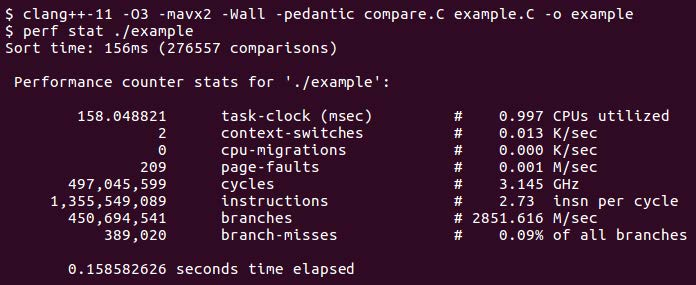
\includegraphics[width=0.9\textwidth]{content/1/chapter2/images/6.jpg}\\
圖 2.6
\end{center}

從圖2.6中可以看到,編譯不需要任何特殊選項或工具。程序由分析器執行,\texttt{stat}選項告訴分析器顯示在程序運行期間,硬件性能計數器中累積的計數值。本例中,程序運行了158毫秒(與程序本身打印的時間一致),並執行了13億多條指令。還顯示了其他幾個計數器,如“頁面錯誤”和“分支”。這些計數器是什麼,還有哪些計數器可用?

事實證明,現代CPU可以收集不同類型事件的統計信息,但一次只能收集幾種類型的事件。前面的例子中,展示了8個計數器,因此可以假設這個CPU有8個獨立的計數器。以前,每個計數器都會分配到一個事件類型中。分析器本身可以列出所有已知的事件,並可以計數:

%\hspace*{\fill} \\ %插入空行
\begin{center}
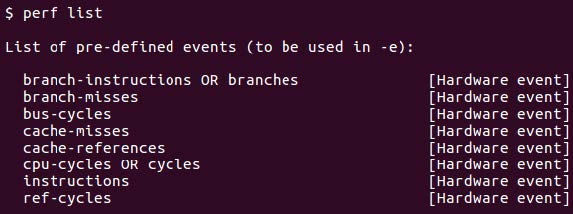
\includegraphics[width=0.9\textwidth]{content/1/chapter2/images/7.jpg}\\
圖 2.7
\end{center}

圖2.7中的列表是不完整的,可用的計數器因CPU而異(如果使用虛擬機,則在類型和配置上有所不同)。圖2.6中的結果只是默認配置的計數器收集的,我們還可以選擇其他的計數器進行配置:

%\hspace*{\fill} \\ %插入空行
\begin{center}
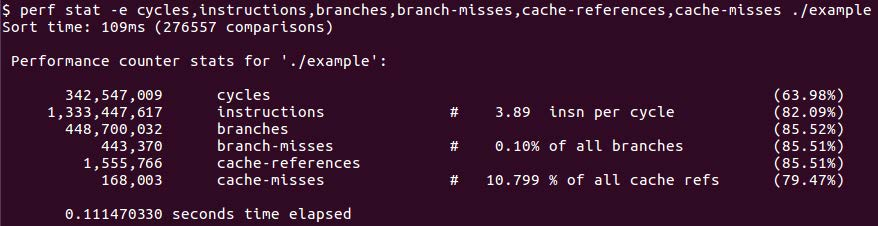
\includegraphics[width=0.9\textwidth]{content/1/chapter2/images/8.jpg}\\
圖 2.8
\end{center}

圖2.8中,我們可以測量CPU週期和指令,以及分支、分支缺失、緩存引用和緩存缺失。下一章將詳細解釋這些計數器和其相應的監視事件。

簡單地說,週期時間是CPU頻率的倒數,所以一個3GHz的CPU每秒可以運行30億個週期。大多數CPU的頻率是可變的,這使得測量變得更復雜了。因此,為了精確的分析和進行基準測試,建議禁用省電模式和其他會讓CPU時鐘變化的功能。指令計數器測量處理器執行指令的數量,CPU平均每週期可以執行四條指令。

“分支”是條件指令:每個帶有條件的\texttt{if}語句和每個\texttt{for}循環都會生成多條這樣的指令。分支缺失在下一章進行解釋,現在只能說這是一個性能開銷大,而且不受歡迎的事件。

“緩存引用”計算CPU需要從內存中讀取的次數。大多數時候是一段數據,比如:字符串中的一個字符。根據處理器和內存的狀態,這個取回可以非常快,也可以非常慢。慢的話會認為是“緩存丟失”(“慢”是一個相對概念:相對於3GHz的處理器速度,1微秒是一個很長的時間)。內存層次結構將在後面的章節進行解釋,而且緩存丟失也是一個性能開銷特別大的事件。

理解了CPU和內存的工作方式後,就能夠使用這些指標來衡量程序的總體效率,並確定哪些因素限制了程序的性能。

目前為止,我們只看到了整個項目的測量結果。圖2.8中表明哪些事件拖累了代碼的性能,例如:如果現在接受“緩存丟失”對性能不利的觀點,可以推斷出這段代碼的主要問題是低效的內存訪問(十分之一的內存訪問是緩慢的)。然而,代碼具體是哪部分導致了較差的性能,這種類型的數據並沒有展示出來。為此,不僅需要在程序執行前後收集數據,還需要在程序執行期間收集數據。來看看如何用\texttt{perf}來收集這些信息。

\subsubsubsection{2.4.2\hspace{0.2cm}使用perf進行詳細分析}

\texttt{perf}分析器將硬件計數器與基於時間採樣結合,記錄正在運行程序的性能情況。對於每個示例,記錄程序計數器的位置(要執行的指令的地址)和需要查看的性能計數器。運行後對數據進行分析,包含大多數的函數和代碼行的執行時間。

分析器的數據收集不會特別複雜。在運行時,收集指令地址轉換為原始源代碼中的行號,程序必須使用調試信息進行編譯。若已經習慣了“優化”和“非優化”這兩種編譯模式,這種編譯器選項的組合可能會出乎意料,這時“優化”和“非優化”都會啟用。啟用後者的原因是,我們需要在生產環境中運行的相同代碼;否則,數據沒什麼無意義。所以需要通過編譯代碼來分析,並使用\texttt{perf record}命令運行分析器:

%\hspace*{\fill} \\ %插入空行
\begin{center}
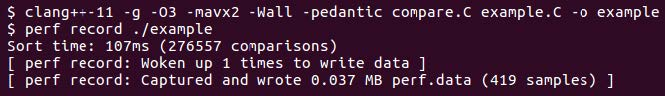
\includegraphics[width=0.9\textwidth]{content/1/chapter2/images/9.jpg}\\
圖 2.9
\end{center}

與\texttt{perf stat}類似,可以指定計數器或一組計數器。但這次,使用默認計數器。我們沒有具體說明採樣的頻率,也使用默認值。採樣頻率可以顯式指定,例如:\texttt{perf record -c 1000}即記錄每秒1000個樣本。

運行程序後,屏幕輸出包括常規輸出和分析器的信息。上一個例子中,分析樣本已經捕獲到名為\texttt{perf.data}的文件中(這是也可以修改)。為了將文件中的數據可視化,需要使用數據分析工具,就是\texttt{perf report}。運行此命令後,界面如下所示:

%\hspace*{\fill} \\ %插入空行
\begin{center}
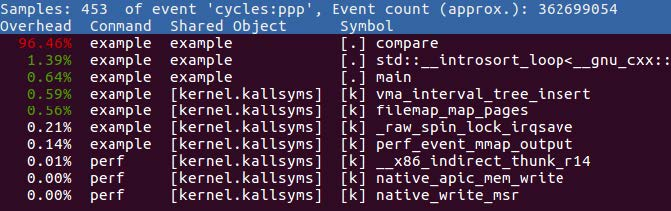
\includegraphics[width=0.9\textwidth]{content/1/chapter2/images/10.jpg}\\
圖 2.10
\end{center}

這就是對數據的分析,按函數執行時間佔總時長佔比進行排序。可以深入到函數內部,瞭解哪一行代碼執行的時間最長:

%\hspace*{\fill} \\ %插入空行
\begin{center}
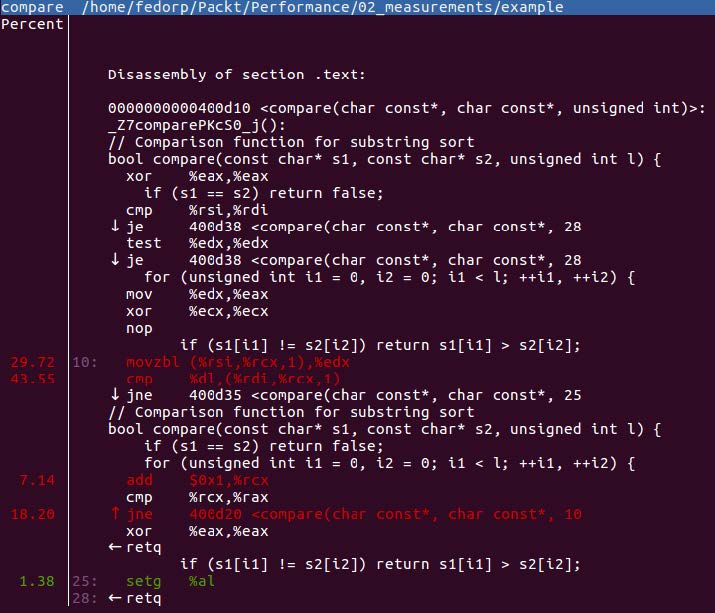
\includegraphics[width=0.9\textwidth]{content/1/chapter2/images/11.jpg}\\
圖 2.11
\end{center}

圖2.11左邊的數字是每一行執行時間的百分比。這條“線”說明瞭什麼?其顯示了源代碼和產生的彙編指令,執行時間計數器與每個硬件指令相關聯(這是CPU執行的指令,所以這是可計數的)。編譯後的代碼可以和源代碼進行關聯,這種關聯是由分析器使用調試信息建立的。然而,因為對代碼進行了優化,所以這種對應並不準確。編譯器在編譯時對原始代碼進行優化,這些優化會導致代碼重排,並可能改變計算的方式。即使在這個簡單的例子中也可以看到一個很詭異的現象:下面的源碼行出現了兩次。

\begin{lstlisting}[style=styleCXX]
if (s1 == s2) return false;
\end{lstlisting}

原因是這一行生成的指令並不都在同一個地方;優化器將它們與來自其他行的指令重新排序。因為這兩條指令最初由它生成,所以分析器將這行源碼顯示在兩條機器指令附近。

即使不看彙編程序,我們也可以知道,時間花在比較字符和運行循環上,以下兩行源碼佔用了大部分時間:

\begin{lstlisting}[style=styleCXX]
for (unsigned int i1 = 0, i2 = 0; i1 < l; ++i1, ++i2) {
	if (s1[i1] != s2[i2]) return s1[i1] > s2[i2];
\end{lstlisting}

為了充分利用這些數據,至少有助於理解當前使用平臺(在我們的例子中是x86 CPU)的彙編語言。分析器還提供了一些有助於分析的工具,例如:通過將光標放在\texttt{jne}(如果不是等於的話跳轉)指令上,可以跳轉到哪裡,以及與跳轉相關的條件:

%\hspace*{\fill} \\ %插入空行
\begin{center}
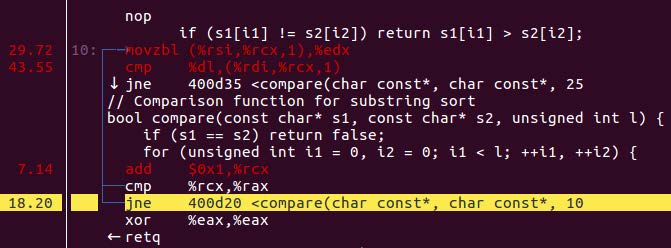
\includegraphics[width=0.9\textwidth]{content/1/chapter2/images/12.jpg}\\
圖 2.12
\end{center}

這看起來會重複跳轉最後幾行代碼,所以跳轉前面的\texttt{cmp}(compare)指令必須是\texttt{i1 < l},跳轉和比較總共佔了執行時間的18\%,所以之前對(不必要的)比較操作的關注是合理的。

\texttt{perf}分析器有很多的選項和功能來分析、過濾和合並結果,可以從其文檔中瞭解更具體的內容(這個分析器也有幾個GUI前端)。接下來,我們將快速瞭解另一個分析器,來自谷歌的性能工具。

\subsubsubsection{2.4.3\hspace{0.2cm}谷歌的性能分析器}

谷歌CPU分析器使用硬件性能計數器,也需要代碼的鏈接時按插指令(但編譯時不需要)。要準備代碼進行分析,必須將與分析器的庫進行鏈接:

%\hspace*{\fill} \\ %插入空行
\begin{center}

\includegraphics[width=0.9\textwidth]{content/1/chapter2/images/13.jpg}\\
圖 2.13
\end{center}

圖2.13中,這個庫是由\texttt{-lprofiler}指定的。與perf不同,這個分析器不需要任何特殊工具來調用程序,因為相應的代碼已經鏈接到可執行文件中。可檢測的可執行文件不會自動開始分析,必須通過設置環境變量\textit{CPUPROFILE}為要存儲結果的文件指定路徑。其他選項也通過環境變量來控制(不用命令行選項),例如:通過變量\texttt{CPUPROFILE\_FREQUENCY}設置每秒採樣數:

%\hspace*{\fill} \\ %插入空行
\begin{center}
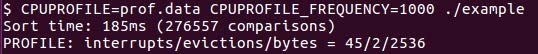
\includegraphics[width=0.9\textwidth]{content/1/chapter2/images/14.jpg}\\
圖 2.14
\end{center}

同樣,我們看到了程序本身和分析器的輸出,並得到了必要的數據文件。該分析器有交互式和批處理兩種模式,其交互模式是一個簡單的文本界面:

%\hspace*{\fill} \\ %插入空行
\begin{center}
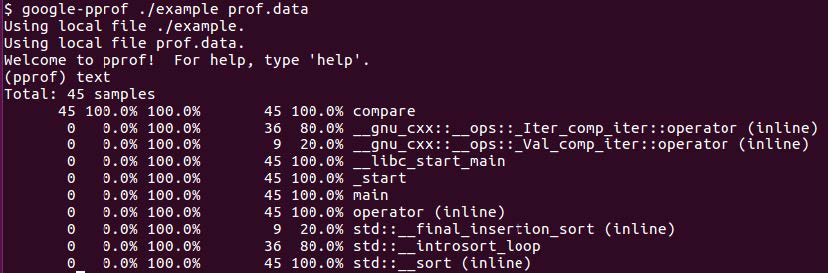
\includegraphics[width=0.9\textwidth]{content/1/chapter2/images/15.jpg}\\
圖 2.15
\end{center}

只需以可執行文件和數據文件的名稱作為參數運行\texttt{google-pprof}(通常只安裝為\texttt{pprof}),就會彈出命令提示符。這裡,可以得到用執行時間百分比標註的函數信息,可以在源代碼級別進一步分析程序性能:

%\hspace*{\fill} \\ %插入空行
\begin{center}
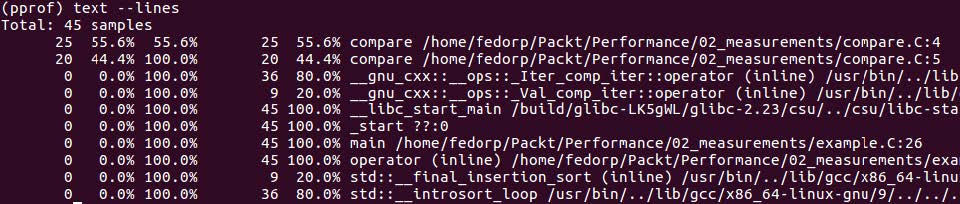
\includegraphics[width=0.9\textwidth]{content/1/chapter2/images/16.jpg}\\
圖 2.16
\end{center}

這個分析器採用了不同的方法,並且不會立即深入到機器代碼中(儘管也可以生成帶註釋的彙編碼)。儘管表面上的看起來簡單,其實不然。前面提到的優化警告仍然存在,編譯器仍然會對代碼進行優化(指令重排)。

由於作者實現的方法不同,不同的分析器就有不同的優缺點。為了不將這一章變成分析器手冊,我們將在本節的其餘部分展示在收集和分析數據文件時,可能遇到的問題。

\subsubsubsection{2.4.4\hspace{0.2cm}使用調用圖進行分析}

目前為止,簡單示例規避了實際中在每個程序中都會遇到的問題。我們看到比較函數佔了大部分的執行時間,這樣就能立即知道程序的哪個部分非常耗時,因為這個函數只有這一行代碼。

現實中的程序都沒有這麼簡單,編寫函數的主要原因是便於重用。顯然,許多函數在多個位置上都有調用,有些是多次,有些可能只有幾次,不同的調用通常會使用不同的參數。這樣的話,只知道哪個函數花費大量時間就不夠了,還需要知道使用這個函數的上下文(畢竟,最有效的優化可能是少調用性能開銷大的函數)。

需要的是一個數據文件,需要報告在每個函數和每行代碼中花費了多少時間,而且還顯式每個調用鏈中花費了多少時間。分析器通常使用調用圖來顯示這些信息。在圖中,調用者和被調用者是節點,而調用是邊。

首先,我們修改示例,在多個位置調用某個函數。讓我們從兩種類型的\texttt{sort}調用開始:

\hspace*{\fill} \\ %插入空行
\noindent
\textbf{05\_compare\_timer.C}
\begin{lstlisting}[style=styleCXX]
std::sort(vs.begin(), vs.end(),
  [&](const char* a, const char* b) {
	++count; return compare1(a, b, L); });
std::sort(vs.begin(), vs.end(),
  [&](const char* a, const char* b) {
	++count; return compare2(a, b, L); });
\end{lstlisting}

調用僅在比較函數中不同。我們的例子中,第一個比較函數與前面相同,第二個比較函數的順序相反。兩個函數對子字符串的循環與原來的比較函數相同:

\hspace*{\fill} \\ %插入空行
\noindent
\textbf{05\_compare\_timer.C}
\begin{lstlisting}[style=styleCXX]
bool compare1(const char* s1, const char* s2, unsigned int l) {
	if (s1 == s2) return false;
	for (unsigned int i1 = 0, i2 = 0; i1 < l; ++i1, ++i2) {
		int res = compare(s1[i1], s2[i2]);
		if (res != 0) return res > 0;
	}
	return false;
}
bool compare2(const char* s1, const char* s2, unsigned int l) {
	if (s1 == s2) return false;
	for (unsigned int i1 = 0, i2 = 0; i1 < l; ++i1, ++i2) {
		int res = compare(s1[i1], s2[i2]);
		if (res != 0) return res < 0;
	}
	return false;
}
\end{lstlisting}

兩個函數都使用相同的公共函數來比較每個字符:

\begin{lstlisting}[style=styleCXX]
int compare(char c1, char c2) {
	if (c1 > c2) return 1;
	if (c1 < c2) return -1;
	return 0;
}
\end{lstlisting}

實際程序中不會這樣做,如果希望避免由於重複循環而造成的代碼重複,那麼應該編寫一個參數化比較字符的函數。無論如何,我們都不想離起始示例太遠,希望代碼保持簡單,以便分析結果。

我們已經準備好生成一個調用圖,將顯示如何在兩個排序調用之間分割字符比較的開銷。使用過的兩種分析器都可以生成調用圖;在本節中,將使用谷歌分析器。分析器收集的數據已經包含了調用鏈信息,只是還沒把它可視化。

我們編譯代碼,並運行分析器(簡單起見,我們把每個函數分別放在不同的源文件中):

%\hspace*{\fill} \\ %插入空行
\begin{center}
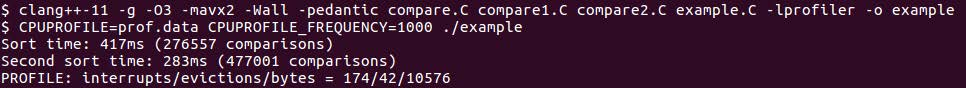
\includegraphics[width=0.9\textwidth]{content/1/chapter2/images/17.jpg}\\
圖 2.17
\end{center}

分析器可以以幾種不同的格式(Postscript、GIF、PDF等)顯示調用圖,例如:要生成PDF輸出,需要運行以下命令:

\begin{tcblisting}{commandshell={}}
google-pprof --pdf ./example prof.data > prof.pdf
\end{tcblisting}

我們感興趣的信息在調用圖的底部:

%\hspace*{\fill} \\ %插入空行
\begin{center}
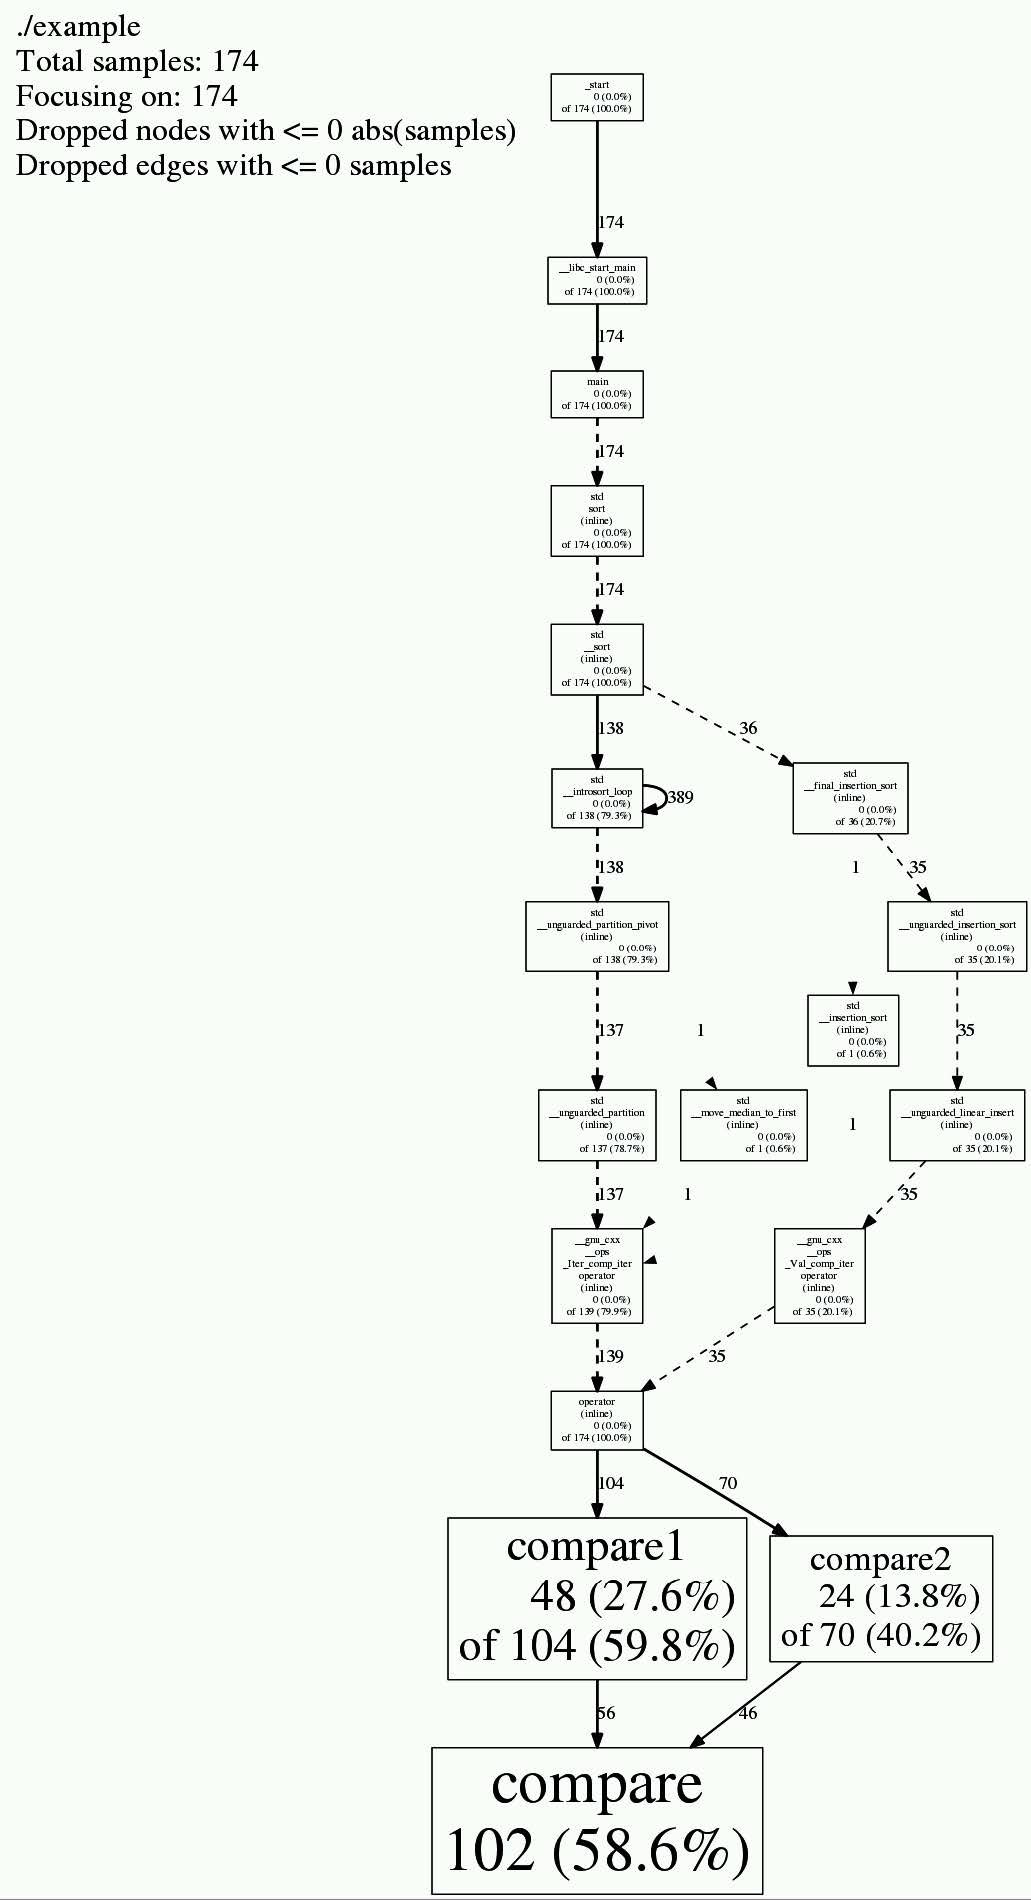
\includegraphics[width=0.6\textwidth]{content/1/chapter2/images/18.jpg}\\
圖 2.18
\end{center}

如圖2.18所示,\texttt{compare()}函數有兩個調用函數,佔總執行時間的58.6\%。這兩個調用函數中,\texttt{compare1()}函數比\texttt{compare2()}函數調用的次數稍多一些;前者佔執行時間的27.6\%(或59.8\%的\texttt{compare()}耗時),後者佔13.8\%的時間(或40.2\%的\texttt{compare()}耗時)。

基本調用圖通常足以確定問題的調用鏈,並選擇程序需要進一步探索的區域。分析工具還具有更高級的功能,例如:過濾函數名、合併結果等。掌握所選工具的特性可以區分實際和假設。解析性能數據文件可能會比較複雜,原因有很多:一些是由於工具的限制,另一些是更偏向於原理性的解釋。下一節中,我們將討論後一個原因:為了使指標具有相關性,測試必須在完全優化的代碼上進行。

\subsubsubsection{2.4.5\hspace{0.2cm}優化和內聯}

解析性能數據文件時,我們已經看到了編譯器優化是如何攪渾這趟水的:所有的數據文件都是同時生成,並在已編譯的機器碼上完成的,而我們看到的是程序的源代碼。由於編譯器優化,這兩種形式之間的關係會變得模糊不清。就重新排列源代碼而言,最積極的優化方式是函數的編譯時內聯。

內聯要求函數的源代碼在調用點是可見的。為了演示,必須將整個源碼合併到一個文件中:

\hspace*{\fill} \\ %插入空行
\noindent
\textbf{02\_substring\_sort.C}
\begin{lstlisting}[style=styleCXX]
bool compare(const char* s1, const char* s2, unsigned int l) {
	if (s1 == s2) return false;
	for (unsigned int i1 = 0, i2 = 0; i1 < l; ++i1, ++i2) {
		if (s1[i1] != s2[i2]) return s1[i1] > s2[i2];
	}
	return false;
}
int main() {
	…
	size_t count = 0;
	std::sort(vs.begin(), vs.end(),
	  [&](const char* a, const char* b) {
		++count; return compare(a, b, L); });
}
\end{lstlisting}

現在編譯器可以(很可能會)在排序使用比較的地方生成機器代碼,而不是調用外部函數。這樣的內聯是有效的優化方式,當然這種情況經常發生,並不僅僅發生在同一個文件的函數上。更常見的情況是,內聯會影響只包含頭文件的函數(其整個實現都在頭文件中),例如:前面的代碼中,對\texttt{std::sort}的調用(看起來像函數調用)肯定是內聯的,因為\texttt{std::sort}是模板函數,其整個實現都在頭文件中。

我們之前使用的分析器工具是如何處理內聯代碼的,為帶註釋的源代碼運行谷歌分析器會產生以下報告:

%\hspace*{\fill} \\ %插入空行
\begin{center}
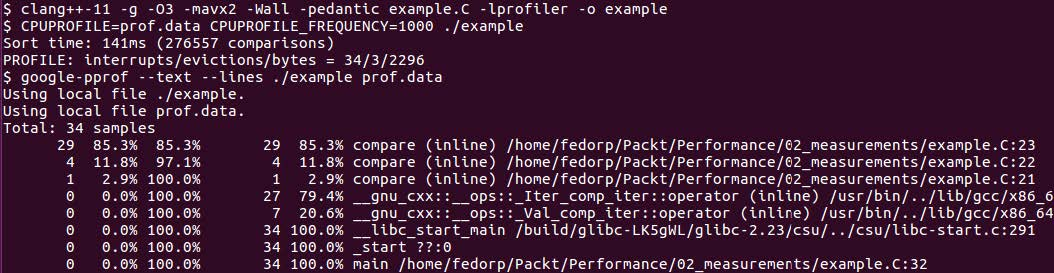
\includegraphics[width=0.9\textwidth]{content/1/chapter2/images/19.jpg}\\
圖 2.19
\end{center}

看來分析器知道\texttt{compare()}是內聯的,但仍然會顯示其原始名稱。源代碼中的行對應的是函數代碼寫入的位置,而不是函數調用的位置,例如:第23行是這樣的:

\begin{lstlisting}[style=styleCXX]
if (s1[i1] != s2[i2]) return s1[i1] > s2[i2];
\end{lstlisting}

另一方面,perf分析器很難顯示內聯函數:

%\hspace*{\fill} \\ %插入空行
\begin{center}
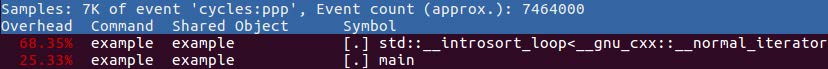
\includegraphics[width=0.9\textwidth]{content/1/chapter2/images/20.jpg}\\
圖 2.20
\end{center}

這裡,我們可以看到時間似乎花在排序代碼和主程序本身上。然而,檢查帶註釋的彙編碼可以看到,由\texttt{compare()}函數源碼生成的代碼,仍佔了大多數的執行時間:

%\hspace*{\fill} \\ %插入空行
\begin{center}
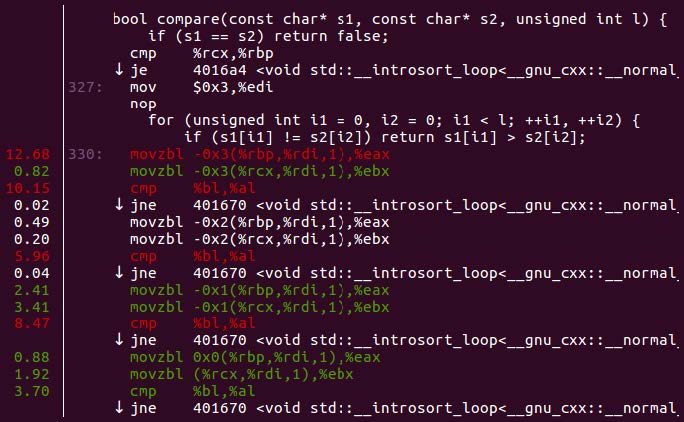
\includegraphics[width=0.9\textwidth]{content/1/chapter2/images/21.jpg}\\
圖 2.21
\end{center}

不幸的是,沒有簡單的方法可以撤消優化對性能數據文件的影響。分析內聯、代碼重新排序和其他轉換的性能,將會轉化為一種隨實踐而發展的技能。現在,給出一些對分析的建議。

\subsubsubsection{2.4.6\hspace{0.2cm}分析建議}

人們可能很容易認為,分析是滿足所有性能測試需求的最終解決方案:在分析器下運行整個程序,收集所有數據,並對代碼中發生的一切進行分析。不幸的是,這種方法很少奏效。有時,工具的限制會成為障礙。通常,處理大量信息的複雜性太大了。那麼,應該如何有效地進行分析呢?

建議是首先收集高級信息,然後進行細化。解析大型模塊之間執行時間的數據,可能是一個很好的起點。另一方面,如果這些模塊用於基準測試,並且有計時器對所有主要執行步驟進行記錄,那麼就可以收到到這些信息了。若沒有這樣的工具,初始的數據文件為這些步驟提供了很好的建議,所以可以現在考慮添加基準測試的工具,以便下次使用,沒人會認為一次性就能解決所有的問題吧?

有了基準測試結果和數據的概要,可能會遇到以下幾個情況。這個數據文件會指向一些簡單的結果,比如:一個花99\%時間做列表的函數。當第一次編寫代碼時,沒有人期望數組的長度超過10個元素,所以只持續了一段時間,然後所有人都忘記了這段代碼,直到它出現在數據文件上。

更有可能的是,數據概要文件將引導找到一些大型函數或模塊。必須迭代、創建專注於程序有趣部分的測試,並更詳細地分析更小的代碼部分。一些基準測試數據也有助於解釋數據文件:雖然數據文件會說明在給定函數或循環中花費了多少時間,但它不會計算循環迭代或跟蹤if-else。大多數分析器都能計數函數調用,所以一個好的模塊化代碼比一個龐大的代碼堆更容易分析。

如果需要收集和細化數據文件,數據會將分析者的注意力集中到代碼性能的關鍵部分。這也是可能會陷入錯誤的地方:當專注於過慢的代碼時,可能會直接優化它,而不考慮其他的情況,例如:數據文件顯示某個特定循環在內存分配上花費的時間最多。當決定需要更高效的內存分配時,請考慮是否需要在循環的每個迭代中分配和回收內存。使慢代碼變快的最好方法通常是減少調用頻率。這可能需要一個不同的算法,或者一個更有效的實現。

通常情況下必須進行計算,這是代碼中性能至關重要的部分,加快程序速度的唯一方法是使代碼更快。所以必須嘗試不同的方法來進行優化,看看哪種方法最有效。可以直接在程序中實現,但這通常是一種浪費時間的方法,會顯著降低工作效率。理想情況下,可以快速試驗針對特定問題的解決方案,從而提出不同實現或不同算法。這裡,可以利用第三種方法來收集性能數據,即微基準測試。













